\subsection{Karrusel: System uden potentiel energi} \label{sec:Karrusel}
\begin{figure}
	\centering
	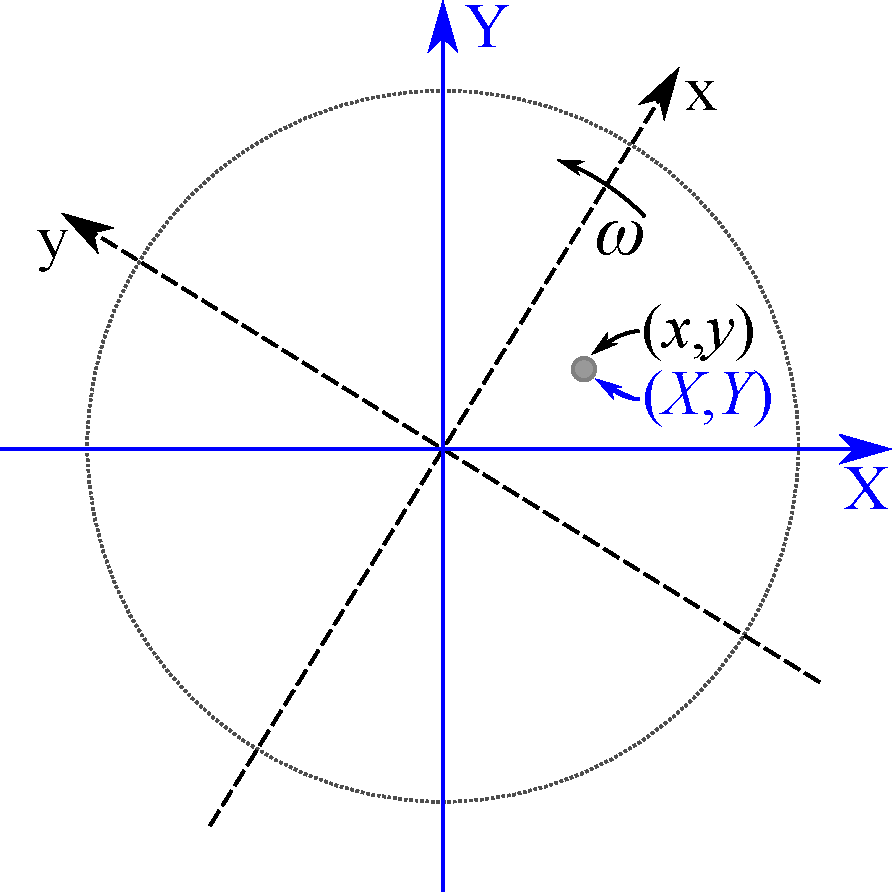
\includegraphics[width=0.4\columnwidth]{figurer/Karussel.pdf}
	\caption{Roterende karussel. Det stiplede sorte koordinatsystem roterer med karussellen således, at et punkt på karrusellen i dette koordinatsystem altid har koordinaterne $(x,y)$. I det fastlåste blå koordinatsystem roterer karussellen, hvorfor førnævnte punkt i dette koordinatsystem vil have skiftende koordinater, der er givet ved $(X,Y)$, \cref{mek:eq:Karussel_X_Y_koordinater}.}
	\label{mek:fig:Karussel}
\end{figure}

Ovenfor har der været kigget på systemer, der har haft både kinetisk og potentiel energi, hvorfor der nu ses på et system uden potentiel energi: En karrusel, \cref{mek:fig:Karussel}.

\noindentm
I dette system betragtes en partikel med masse $m$, der bevæger sig relativt til et roterende koordinatsystem, som følger karrusellen (stiplet koordinatsystem i \cref{mek:fig:Karussel}). I dette koordinatsystem har partiklen koordinaterne $(x,y)$. Betragtes dette system ud fra et stillestående koordinatsystem (blåt koordinatsystem i \cref{mek:fig:Karussel}) med samme origo, vil karrusellen rotere med en vinkelhastighed $\omega$. I dette koordinatsystem vil partiklens koordinater være $(X,Y)$. Sammenhængen mellem partiklens koordinater i de to koordinatsystemer er givet ved\footnote{Dette fås ved at gange en rotationsmatrix på stedvektoren $h$, hvilket her bare tages for gode varer.}
%
\begin{equation} \label{mek:eq:Karussel_X_Y_koordinater}
	\begin{aligned}
		X &= x \cos(\omega t) - y \sin(\omega t) \: , \\
		Y &= x \sin(\omega t) + y \cos(\omega t) \: .
	\end{aligned}
\end{equation}
%
For at finde den kinetiske energi, beregnes de afledede af koordinaterne, hvilket giver
%
\begin{equation}
	\begin{aligned}
		\dot{X} &= \dot{x} \cos(\omega t) - \omega x \sin(\omega t) - \dot{y} \sin(\omega t) - \omega y \cos(\omega t) \: , \\
		\dot{Y} &= \dot{x} \sin(\omega t) + \omega x \cos(\omega t) + \dot{y} \cos(\omega t) - \omega y \sin(\omega t) \: .
	\end{aligned}
\end{equation}
%
Hernæst beregnes summen af de kvadrerede $\dot{X}$- og $\dot{Y}$-koordinater:
%
\begin{align} \label{mek:eq:KarusselHastighed}
	\dot{X}^2 + \dot{Y}^2 &= \dot{x}^2 + \omega^2 x^2 + \dot{y}^2 + \omega^2 y^2 - \dot{x}y \omega + x \dot{y} \omega + x \dot{y} \omega - \dot{x} y \omega \nonumber \\
	&= \dot{x}^2 - \dot{y}^2 + \omega(x^2 + y^2) + 2 \omega (x \dot{y} - \dot{x} y) \: .
\end{align}
%
De første fire led i \cref{mek:eq:KarusselHastighed} fremkommer på samme måde, og her forklares blot fremkomsten af $\dot{x}^2$ leddet: Kvadreres $\dot{X}$ og $\dot{Y}$ fremkommer led som er kvadrerede, for eksempel
%
\begin{align*}
	[\dot{x} \cos(\omega t)]^2 &= \dot{x}^2 \cos^2(\omega t) \: , \\
	[\dot{x} \sin(\omega t)]^2 &= \dot{x}^2 \sin^2(\omega t) \: .
\end{align*}
%
Siden summen af de kvadredede $\dot{X}$- og $\dot{Y}$-koordinater beregnes, vil man få
\begin{align*}
	\dot{x}^2 \cos^2(\omega t) + \dot{x}^2 \sin^2(\omega t) &= \dot{x}^2 (\cos^2(\omega t) + \sin^2(\omega t)) = \dot{x}^2 \: ,
\end{align*}
%
da $\cos^2(\omega t) + \sin^2(\omega t) = 1$, hvilket kaldes grundrelationen.

\noindent
For de resterende fire led er der også gjort brug af grundrelationen, men her blot mellem krydsleddene: Tages et eksempel kan det ses at
%
\begin{align*}
	\left[\dot{x}\cos(\omega t)\right] \left[-\omega y\cos(\omega t)\right] &= -\dot{x}\omega y \cos^2(\omega t) \: , \\
	\left[\dot{x}\sin(\omega t)\right] \left[-\omega y\sin(\omega t)\right] &= -\dot{x}\omega y \sin^2(\omega t) \: .
\end{align*}
%
Sammenlægges disse to led fås
%
\begin{align*}
	-\dot{x}\omega y \cos^2(\omega t) -\dot{x}\omega y \sin^2(\omega t) &= -\dot{x}\omega y \left(\cos^2(\omega t) + \sin^2(\omega t)\right) = -\dot{x}\omega y \: .
\end{align*}

\noindent
De resterende krydsled fra sammenlægningen $\dot{X}$ og $\dot{Y}$ går ud med hinanden, eksempelvis
%
\begin{align*}
	\left[\dot{x}\cos(\omega t)\right] \left[-\omega x \sin(\omega t)\right] &= -\dot{x}x\omega\cos(\omega t)\sin(\omega t) \: , \\
	\left[\dot{x}\sin(\omega t)\right] \left[\omega x \cos(\omega t)\right] &= \dot{x}x\omega\cos(\omega t)\sin(\omega t) \: ,
\end{align*}
%
hvorfor disse ikke indgår i \cref{mek:eq:KarusselHastighed}.

\noindent
Ud fra \cref{mek:eq:KarusselHastighed} fås følgende kinetisk energi
%
\begin{align}
	K &= \frac{1}{2} m \left(\dot{X}^2 + \dot{Y}\right) = \frac{1}{2} m \left[ \dot{x}^2 - \dot{y}^2 + \omega(x^2 + y^2) + 2 \omega (x \dot{y} - \dot{x} y) \right] \: ,
\end{align}
%
og da der ingen potentiel energi er i systemet, bliver Lagrangefunktionen
%
\begin{align}
	L &= K = \frac{1}{2} m \left[ \dot{x}^2 - \dot{y}^2 + \omega(x^2 + y^2) + 2 \omega (x \dot{y} - \dot{x} y) \right] \: .
\end{align}
%
Fra denne Lagrangefunktion kan følgende partielt afledede med hensyn til $x$ og $\dot{x}$ findes
%
\begin{align}
	\pdv{L}{x} &= \frac{1}{2} m \left[ 2\omega^2x + 2\omega \dot{y} \right] = m \left( \omega^2x + \omega \dot{y} \right) \: , \\
	\pdv{L}{\dot{x}} &= \frac{1}{2} m \left[ 2 \dot{x} - 2\omega y \right] = m \left( \dot{x} - \omega y \right) \: , \\
	 \dv{}{t} \left( \pdv{L}{\dot{x}} \right) &= m \left( \ddot{x} - \omega \dot{y} \right) \: ,
\end{align}
%
hvorved Euler-Lagrangeligningen bliver
%
\begin{align}
	\pdv{L}{x} &= \dv{}{t} \left( \pdv{L}{\dot{x}} \right) \nonumber \\
	\Rightarrow m \left( \omega^2 x + \omega \dot{y} \right) &= m \left( \ddot{x} - \omega \dot{y} \right) \: ,
\end{align}
%
så bevægelsesligningen bliver
%
\begin{align} \label{mek:eq:xKarrusel}
	\ddot{x} &= \omega^2x + 2 \omega \dot{y} \: .
\end{align}

\noindent
For $y$ og $\dot{y}$ bliver de partielt afledede
%
\begin{align}
	\pdv{L}{y} &= \frac{1}{2} \left[ 2 \omega^2y - 2\omega\dot{x} \right] = m \left( \omega^2y - \omega \dot{x} \right) \: , \\
	\pdv{L}{\dot{y}} &= \frac{1}{2} \left[2 \dot{y} + 2 \omega x \right] = m \left( \dot{y} + \omega x \right) \: , \\
	\dv{}{t} \left(\pdv{L}{\dot{y}}\right) &= m \left( \ddot{y} - \omega \dot{x} \right) \: ,
\end{align}
%
hvorved Euler-Lagrangeligningen bliver
%
\begin{align}
	\pdv{L}{y} &= \dv{}{t} \left(\pdv{L}{\dot{y}}\right) \nonumber \\
	\Rightarrow m \left( \omega^2 y-\omega \dv{t} x \right) &= m \left( \ddot{y} - \omega \dot{x} \right) \: ,
\end{align}
%
og der fås følgende bevægelsesligning for partiklen i $y$-retningen
%
\begin{align} \label{mek:eq:yKarrusel}
	\ddot{y} &= \omega^2y - 2 \omega \dot{x} \: .
\end{align}

\noindent
Det kan med nogle lettere bøvlede udregninger vises, at Corioliskraften og centrifugalkraften er givet som
%
\begin{equation} \label{mek:eq:FiktiveKraefter}
\begin{aligned}
	\va{F}_\mathrm{cor} &= 2m\dot{\va{r}}\times\va{\Omega} \: , \\
	\va{F}_\mathrm{cf} &= m(\va{\Omega} \times \va{r}) \times \va{\Omega} \: ,
\end{aligned}
\end{equation}
%
hvor $\va{r}$ er stedvektoren for det legeme, som kræfterne påvirker, og $\va{\Omega}$ er vinkelhastighedsvektoren for det roterende koordinatsystem, som legemet befinder sig i. I dette eksempel roterer karrusellen med vinkelhastigheden $\omega$ omkring $z$-aksen, hvorfor $\va{\Omega} = \omega\vu{z}$. Enhver vektor kan i kartesiske koordinater skrives på formen $\va{r} = x\vu{x} + y\vu{y} + z\vu{z}$. Af denne grund kan Corioliskraften skrives som
%
\begin{equation}
\begin{aligned}
	\va{F}_\mathrm{cor} &= 2m(\dot{x}\vu{x} + \dot{y}\vu{y} + \dot{z}\vu{z}) \times \omega\vu{z} \\
	&= 2m\omega(-\dot{x}\vu{y} + \dot{y}\vu{x}) \: ,
\end{aligned}
\end{equation}
%
og tilsvarende bliver centrifugalkraften
%
\begin{equation}
\begin{aligned}
	\va{F}_\mathrm{cf} &= m[\omega\vu{z} \times (x\vu{x} + y\vu{y} + z\vu{z})] \times \omega\vu{z} \\
	&= m\omega^2[x\vu{y} - y\vu{x}] \times \vu{z} \\
	&= m\omega^2(x\vu{x} + y\vu{y}) \: .
\end{aligned}
\end{equation}
%
Bruges Newtons 2. lov på summen af de fiktive kræfter fås
\begin{align}
	\sum\va{F} &= \va{F}_\mathrm{cor} + \va{F}_\mathrm{cf} \nonumber\\
	\Rightarrow m(\ddot{x}\vu{x} + \ddot{y}\vu{y}) &= 2m\omega(-\dot{x}\vu{y} + \dot{y}\vu{x}) + m\omega^2(x\vu{x} + y\vu{y}) \: ,
\end{align}
%
og samles $x$- og $y$-komposanterne for sig fås
%
\begin{equation}
	\begin{aligned}
		\ddot{x} &= \omega^2x + 2\omega\dot{y} \: , \\
		\ddot{y} &= \omega^2y - 2\omega\dot{x} \: .
	\end{aligned}
\end{equation}
%
Dette er præcis de samme ligninger, som \cref{mek:eq:xKarrusel,mek:eq:yKarrusel}, hvorfor ovenstående kan tænkes som en pseudoudledning af Coriolis- og centrifugalkraften, og det illustrerer også, at de er effekter, som rotationen skaber fra den kinetiske energi i systemet. Grunden til at det ikke er en rigid udledning er, at den er bundet op på det kartesiske koordinatsystem og én specifik rotation. Karrusellen illustrerer dog eksistensen af disse fiktive kræfter, til en vis grad hvor de kommer fra, og den belyser hvad disse kræfter er for nogle størrelser.